\section{Introducción}

En el ámbito global, la Inteligencia Artificial (IA) ha revolucionado diversos sectores, facilitando la toma de decisiones, optimizando procesos y generando soluciones innovadoras para problemas complejos. Particularmente, la IA ha demostrado su potencial en la mejora de sistemas de software diseñados para sectores específicos como lo es el sector de la Seguridad y Salud en el Trabajo (SST), especialmente en contextos como el colombiano que se encuentra en la cúspide de esta revolución tecnológica donde organizaciones como la Corporación Talentum aspiran a liderar iniciativas que generen un impacto positivo en el bienestar laboral.

No obstante, emerge una problemática significativa, que a pesar de los avances en IA, su integración efectiva en soluciones de software orientadas a la SST presenta desafíos que abarcan desde aspectos técnicos hasta cuestiones éticas y de privacidad, y demandan una comprensión profunda y enfoques adaptados para asegurar implementaciones exitosas que realmente beneficien a los usuarios finales y a las organizaciones involucradas.

%Es imperativo abordar esta problemática, dado que las soluciones adecuadas poseen el potencial de transformar cómo las organizaciones gestionan la Seguridad y Salud en el Trabajo. Una implementación efectiva de IA puede facilitar la identificación temprana de riesgos, optimizar respuestas y promover ambientes de trabajo más seguros y saludables. Por lo tanto, resulta esencial establecer estrategias y métodos claros que permitan maximizar los beneficios de la IA en este sector.

En este sentido, se presenta esta propuesta con el propósito de proponer un marco de trabajo para la incorporación de componentes de IA en arquitecturas de software preexistentes con énfasis en SST. El marco de trabajo se compone de prácticas recomendadas, componentes arquitectónicos y criterios para una integración eficaz de una IA, buscando no solo la adaptación técnica sino también el aprovechamiento máximo de la IA para garantizar su impacto y perdurabilidad. En particular, como caso de estudio, se seleccionará un proyecto de desarrollo de software el cual incluya en sus requerimientos funcionales la necesidad de incorporar componentes de IA. La Corporación Talentum es una entidad prominente en la implementación de proyectos gubernamentales en Colombia.

%Para lograr una comprensión profunda y enfrentar la problemática destacada, se realizará una revisión de literatura, fundamentado en una revisión de documentos existentes, el análisis de datos pertinentes y la aplicación de metodologías apropiadas. De esta manera, se proporcionará no solo una base sólida para futuras implementaciones de IA en el ámbito de SST, sino también en productos que incorporen IA en sus requerimientos funcionales.

El resto del documento se estructura de la siguiente manera: la Sección \textbf{Problema} \ref{sec:problema}, se describe la situación problemática y las preguntas específicas. La Sección \textbf{Objetivos del Proyecto} \ref{sec:objetivos} se presentan tanto los objetivos generales como los específicos. De igual manera, se presentan los resultados esperados por cada objetivo específico. La Sección \textbf{Alcance} \ref{sec:alcance} se delimita el alcance del proyecto teniendo en cuenta la sección anterior y el tiempo establecido para la realización de la investigación. La Sección \textbf{Justificación del trabajo de grado} \ref{sec:justificacion} se expone por qué se hace necesario la realización de la investigación. La Sección \textbf{Marco de Referencia y Antecedentes} \ref{sec:marco} incluye las bases teóricas y el estado del arte en la incorporación de IA en desarrollos de software proporcionando un contexto esencial para la investigación. La Sección \textbf{Metodología de la Investigación} \ref{sec:metodologia} expone la metodología adoptada para llevar a cabo la investigación. La Sección \textbf{Recursos a emplear} \ref{sec:recursos} detalla los recursos necesarios para la ejecución del proyecto, incluyendo los recursos humanos, bibliográficos y tecnológicos. La Sección \textbf{Cronograma de Actividades} \ref{sec:cronograma} presenta el cronograma de actividades que guiará el desarrollo de la investigación La Sección \textbf{Referencias Bibliográficas} \ref{sec:bibliografia} lista las referencias bibliográficas que se tuvieron en cuenta durante la ejecución de la presente propuesta de investigación. Finalmente, se presenta un \textbf{Glosario de Términos} \ref{sec:glosario}.\\

La Figura \ref{fig:resumen_proyecto} ayuda a sintetizar de manera visualizar la propuesta de investigación teniendo los aspectos más importantes tales como problema, objetivo y resultados esperados.



\begin{figure}[H]
\centering
\rotatebox{90}{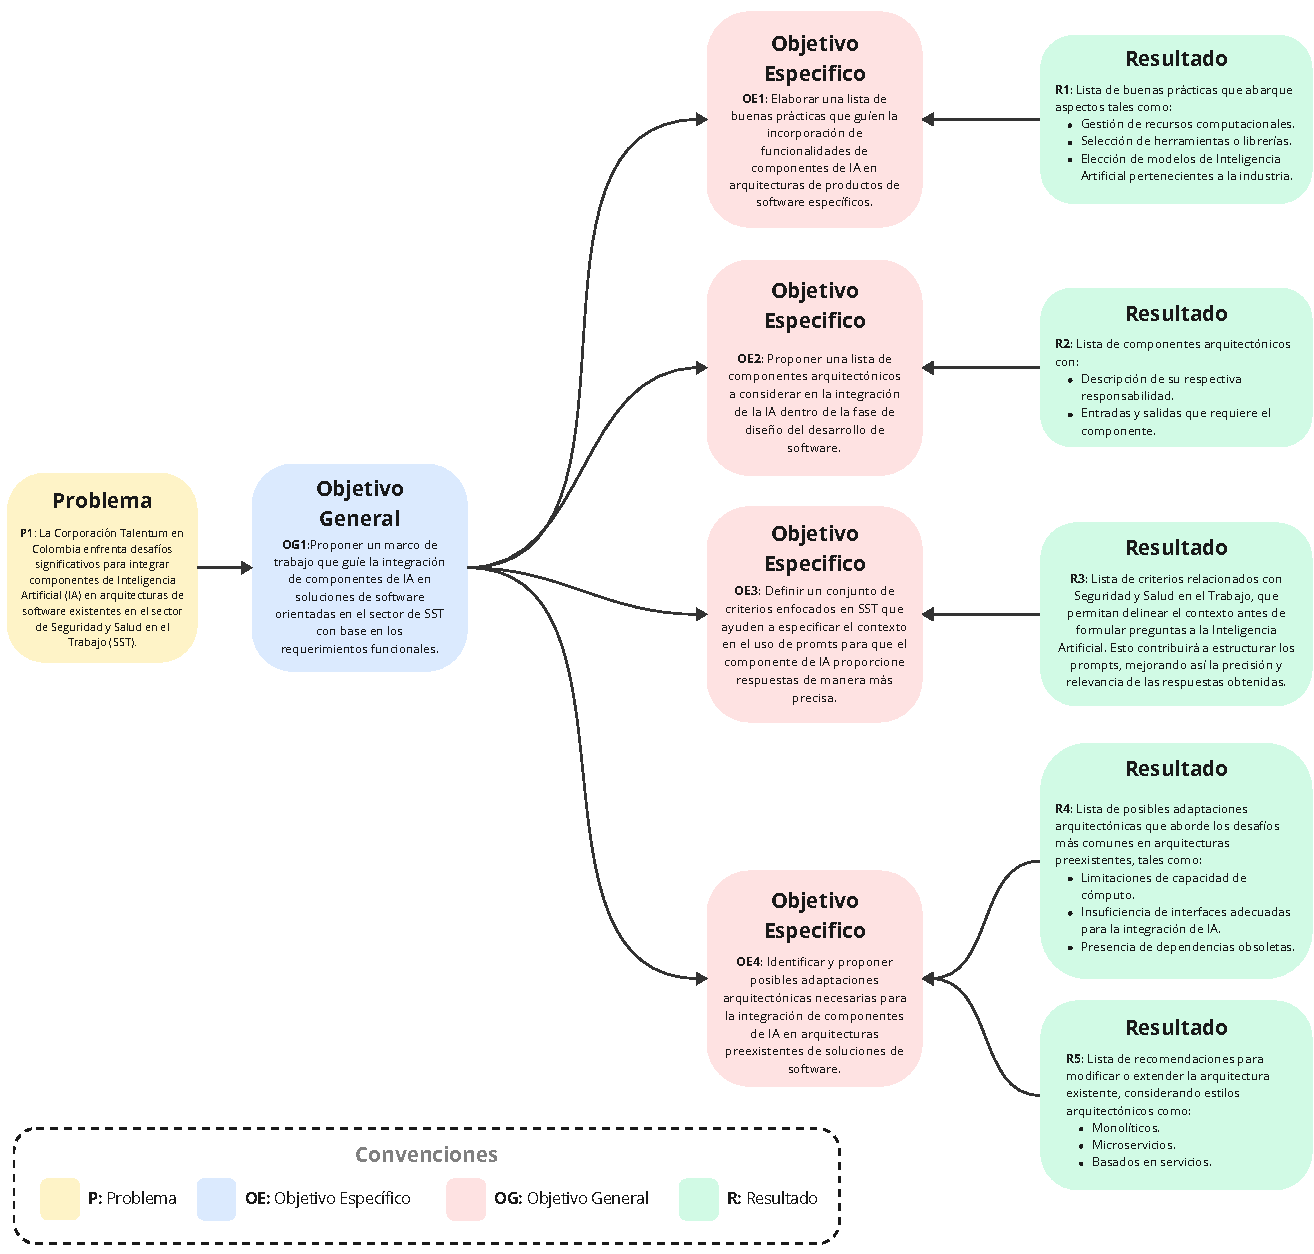
\includegraphics[width=1.15\textwidth]{img/resumen_proyecto.pdf}}
\caption{Diagrama resumen de la propuesta de investigación.}
\label{fig:resumen_proyecto}
\end{figure}